% =====================================================================
%  CUMCM 2026 A 题  药材的烘干问题
%  正文与附录主体（由 paper.tex / paper_electronic.tex 共同 \input）
%  编译：xelatex（必须）
% =====================================================================

\begin{abstract}
中药材热风烘干是典型的「热湿耦合传递 + 相变 + 尺寸收缩」问题。本文以圆柱形药材为
对象，从壳层守恒出发建立温度--水分浓度耦合的轴对称扩散方程组，用保质量的有限体积
/Crank--Nicolson 格式求解，并以多种数值实现与解析解交叉验证。

\textbf{针对问题一}，将长径比 $L/R=12.5$ 的药材简化为无限长圆柱的一维径向问题，由
Fourier 定律与 Fick 定律推得
$\rho c_p\partial_tT=r^{-1}\partial_r(rk\partial_rT)$ 与
$\partial_tC=r^{-1}\partial_r(rD(C)\partial_rC)$，边界取 Robin 条件。先对附件 1 的
实测环境做一阶惯性拟合（$T_{air}$ 的 $R^2=0.9957$，RMSE $=0.336\,^\circ$C），
再以 1600 个控制体、$\Delta t=1$ s 求解：$1800$ s 时中心温度升至
$34.0425\,^\circ$C、表面 $37.1989\,^\circ$C，中心水分浓度仍为 $2.5500$ kg/kg、
表面降至 $1.5109$ kg/kg，截面平均含水由 $2.5500$ 降到 $2.2907$ kg/kg；
干物质质量 $72.57$ g（按附录 2 的 $\rho=820$ kg/m$^3$），1800 s 内脱除水分
$18.71$ g（占初始水量 $10.1\%$）。传质 Fourier 数仅 $0.0222$，
说明该阶段以升温为主、失水集中在表层。

\textbf{针对问题二}，改用附录 3 的变物性关系，并按题意把工艺分为预热平衡
（$0\sim4$ h）与恒温干燥（$t>4$ h，$T_{air}=50.212\,^\circ$C、$C_{air}=0.0509$ kg/kg）
两个阶段。3 h 内中心温升到 $49.9051\,^\circ$C、近似与环境平衡；水分浓度由表及里
依次下降，3 h 时中心 $1.7673$、表面 $1.0083$ kg/kg。

\textbf{针对问题三}，以「处处低于 $0.15$ kg/kg」为判据，指出中心是最后干燥点，
经网格加密与 Richardson 外推得
$\boxed{t_{dry}=205559\ \mathrm{s}=57.10\ \mathrm{h}=2.38\ \mathrm{d}}$，
与题目「一般持续 2--3 天」一致；此时截面平均含水 $0.1232$ kg/kg。

\textbf{针对问题四}，引入物质坐标 $\xi=r/R(t)$，严格导出各向同性收缩下无对流项的
Lagrangian 形式 $\partial_tC=(\xi R^2)^{-1}\partial_\xi(\xi D\partial_\xi C)$，
并用附件 2 的实测 $R(t)$（$2.000\to1.198$ cm）求得
$\boxed{t_{dry}=182765\ \mathrm{s}=50.77\ \mathrm{h}=2.12\ \mathrm{d}}$。
表格距离列取\textbf{当前物理距离} $r$（按 $\xi=r_j/R(t_i)$ 采样、
$r_j>R(t_i)$ 留空）；忽略收缩会把烘干时间高估 $2.5$ 倍。外部校验发现附件 2 的
收缩数据与附录 4 的密度式在干基质量守恒下最大不自洽 $17.8\%$。

\textbf{模型检验}：与 Bessel 级数解析解相比全场最大偏差 $1.0\times10^{-3}$ K、
中心点 $1.2\times10^{-5}$ K；空间与时间收敛阶均为二阶（$N=100\to800$ 误差降
$91$ 倍，$\Delta t=4\to0.25$ s 降 $195$ 倍）。三组数值实现（节点／单元中心有限
体积、直线法）在 $t=2.0\times10^5$ s 的中心含水相差不超过 $0.0066\%$，其中前两者
是两种\textbf{不同的空间离散}；水分守恒残差 $2.1\times10^{-5}$。灵敏度分析表明
\textbf{活化温度 3850 K 主导不确定性}（$\pm2\%\to\pm24\%$），浓度指数次之
（$\pm5\%$）。

\keywords{热湿耦合扩散；变物性；Robin 边界；收缩介质物质坐标；有限体积法；
Richardson 外推；灵敏度分析}
\end{abstract}

% =====================================================================
\section{问题重述}

\subsection{问题背景}

干燥是中药材产地加工与炮制过程中的关键工序，直接决定成品的有效成分保留率、
外观等级与贮藏稳定性；热风烘干因设备简单、成本低，是目前使用最广的干燥方式
之一\cite{li2024,zhang2022}。该过程包含两个阶段：先是\textbf{预热平衡阶段}，药材由环境
温度被加热到接近烘房温度、内部建立起稳定的温度梯度；随后进入\textbf{恒温干燥
阶段}，在近似恒定的温湿度环境下水分由内部迁至表面并被气流带走。工艺参数选择
不当会导致干燥过慢（能耗高、周期长）、表面「结壳」（外干内湿）或温度过高
（破坏热敏性成分），而传统的「试错--检测」优化模式周期长、成本高，因此有必要
用数理模型刻画药材内部温度与水分浓度的时空演化，以预测干燥时长、指导工艺设计。

本题的对象是一根形状近似为圆柱的中药材：长 $25$ cm、半径 $2$ cm，初始温度
$28\,^\circ$C，初始干基含水率 $2.55$ kg/kg。烘房温度与水分浓度的时间序列由
附件 1 给出，药材在干燥过程中的半径变化由附件 2 给出，问题 1--4 所需的物性
经验关系分别由附录 2--4 给出。

\subsection{需要解决的问题}

\begin{itemize}
  \item \textbf{问题一}：建立\textbf{预热平衡阶段}药材温度与水分浓度变化规律的数学模型
  （参数取附录 2），给出 $t=100,300,600,900,1200,1500,1800$ s、$r=0,0.5,1,1.5,2$ cm
  处的温湿度结果，并将 $1800$ s 内每 $1$ s、径向每 $0.1$ cm 的完整结果写入
  \texttt{result1.xlsx}。
  \item \textbf{问题二}：建立\textbf{整个烘干过程}（约 2--3 天）的数学模型，物性统一取
  附录 3，给出 3 h 内每 $0.5$ h、上述五个半径处的结果，并把每 $1$ s、径向每
  $0.1$ cm 的完整结果写入 \texttt{result2.xlsx}。
  \item \textbf{问题三}：以「药材各处水分浓度均低于 $0.15$ kg/kg」为烘干判据，
  确定所需烘干时间（单位 h），给出每 $6$ h、径向每 $0.5$ cm 的水分浓度，并把
  每 $60$ s、径向每 $0.1$ cm 的完整结果写入 \texttt{result3.xlsx}。
  \item \textbf{问题四}：考虑干燥过程中药材因失水而发生的\textbf{尺寸收缩}
  （半径历史见附件 2，物性取附录 4），重新确定烘干时长，给出每 $6$ h、径向每
  $0.5$ cm 的水分浓度（末列为随时间移动的药材表面），并把每 $60$ s、径向每
  $0.1$ cm 的完整结果写入 \texttt{result4.xlsx}。
\end{itemize}

每个问题都需要明确三件事：\textbf{输入}（初始温湿度、烘房环境时间序列、物性关系、
几何尺寸）、\textbf{输出}（规定时刻与位置的温度与水分浓度）、\textbf{判定标准}
（问题 1--2 为数值结果的精度与守恒性；问题 3--4 为「处处低于 $0.15$ kg/kg」这一
判据首次被满足的时刻）。

% =====================================================================
\section{问题分析}

\subsection{为什么是「耦合扩散」而不是「经验干燥曲线」}

中药材的干燥在机理上同时包含三个过程：热量由热风经表面对流进入药材内部
（Fourier 导热）、水分以液态扩散的形式由内部向表面迁移（Fick 扩散）、以及
表面发生的对流传质\cite{mujumdar2014,chaedir2019}。三者由\textbf{材料内部的
温湿度场}耦合在一起：附录的经验关系表明扩散系数 $D$ 同时依赖水分浓度 $C$ 与
温度 $T$（Arrhenius 形式），而 $\rho$、$c_p$、$k$ 又都依赖 $C$。

因此，薄层干燥经验模型（如 Page 模型、Weibull 模型）虽然能拟合整体的含水率--
时间曲线，却\textbf{无法回答本题的核心问题}：题目要求给出「到药材中心不同距离
处」的温度与水分浓度，而经验模型只描述截面平均量、缺少空间分辨率，无法判定
「处处低于 $0.15$ kg/kg」这一内部判据。故必须建立分布参数模型。

理由链可以完整表述为：

\begin{center}
\begin{tabular}{p{0.20\textwidth}p{0.70\textwidth}}
\toprule[1.2pt]
\textbf{环节} & \textbf{内容} \\
\midrule
机理 & 表面受对流换热与对流传质控制；内部受导热与水分扩散控制；物性随 $C,T$ 变化 \\
模型形式 & 轴对称非稳态扩散方程组（抛物型 PDE）+ Robin 边界 + 变系数耦合 \\
可辨识参数 & $\rho,c_p,k,D$ 由附录经验式给出；$h=25\ \mathrm{W/(m^2K)}$、
  $h_m=8\times10^{-7}$ m/s 由附录 2 给出；环境由附件 1 给出 \\
求解方法 & 归一化半径上的有限体积离散 + $\theta$ 法时间推进（$\theta=1/2$ 即
  Crank--Nicolson），三对角线性系统用 LAPACK 带状求解器 \\
可验证性 & 常物性恒环境条件下存在 Bessel 级数解析解；离散格式严格守恒，可做
  水分总量核对；可与降维模型、直线法对照 \\
\bottomrule[1.2pt]
\end{tabular}
\end{center}

\subsection{问题一的分析}

预热平衡阶段只有 $1800$ s。由附录 2 可估算两个特征时间：
热扩散时间 $\tau_T=R^2/\alpha=R^2\rho c_p/k=2369$ s，水分扩散时间
$\tau_D=R^2/D(C_0)=8.1\times10^4$ s。二者相差 34 倍，说明\textbf{在 30 分钟内
温度场会发生显著变化，而水分场只能在表层发生可观测的改变}。这一数量级判断
直接决定了结果形态，也为后续结果合理性检查提供了先验依据。

另一个关键点是\textbf{附件 1 的处理}。附件 1 是带噪声的实测环境序列（241 个
点，采样间隔 60 s），若直接把它作为边界条件会引入阶跃噪声。本文先做一阶惯性
拟合（$T_{air}=T_{set}-(T_{set}-28)e^{-t/\tau_T}$），并把「用拟合曲线」与
「用附件 1 原始插值」两种口径都算过：对 $t_{dry}$ 而言两者只差 $0.12$ h
（$0.2\%$）；但对问题 1 的 30 分钟温度表，拟合曲线在 $60\!\sim\!2300$ s
（$1\!\sim\!38$ min）内\textbf{系统性高于实测，最大偏高 $0.96\,^\circ$C}
（残差滞后 1 阶自相关达 $0.83$，
说明它不只是随机噪声，而是模型形式失配），使表~\ref{tab:p1T} 各值系统性偏高，
最大偏高 $0.52\,^\circ$C（$t=1200$ s、$r=2.0$ cm 处）。本文因此
\textbf{如实报告两种口径}（对照见 10.7 节表~\ref{tab:p1env}）：正文
表~\ref{tab:p1T}、表~\ref{tab:p1C} 取拟合边界，并明确其代价。

\subsection{问题二与问题三的分析}

问题二的时间尺度跃升到 2--3 天，出现了两个新问题。其一，\textbf{物性不再是
常数}：附录 3 的 $D$ 随 $C$ 呈 $\exp(-a/C)$ 下降（$C$ 由 $2.55$ 降到 $0.15$
时降近一个数量级），又对温度呈 $\exp(-3850/T)$ 的强依赖，方程因此\textbf{强
非线性}，干燥后期进入「降速干燥」区，常系数近似会带来系统性偏差。其二，
\textbf{需区分两个工艺阶段}：题目指出两阶段「参数有所不同」，而附件 1 显示
烘房在 4 h 左右达到 $50.2\,^\circ$C 并稳定，故本文取 $0\sim4$ h 为预热平衡
阶段（环境按附件 1 上升）、$t>4$ h 为恒温干燥阶段（$T_{air}=50.212\,^\circ$C、
$C_{air}=0.0509$ kg/kg）。

问题三的关键判断是：\textbf{判据「处处低于 0.15 kg/kg」由中心点最后满足}——
圆柱几何下中心是扩散路径最长的点。本文不预设这一点，而是逐时刻搜索
$\max_r C(r,t)$ 及其位置，用数据确认最大值始终位于中心（8.1 节）。

\subsection{问题四的分析}

尺寸收缩给模型带来两个变化：求解域 $[0,R(t)]$ 是\textbf{移动边界}，且材料点
随收缩向轴心移动。若在固定物理坐标下用移动网格求解，需在方程中显式加入对流项，
边界处理复杂且易引入数值耗散。

本文采用\textbf{物质坐标（Lagrangian）变换} $\xi=r/R(t)$：对各向同性收缩，
每个材料点保持 $\xi$ 不变，由「以固定干基质量为控制体」的守恒推导（5.5 节）
可得水分方程在物质坐标下\textbf{对流项严格为零}：

\[
\frac{\partial C}{\partial t}=\frac{1}{\xi R(t)^2}\frac{\partial}{\partial \xi}
\left(\xi D\frac{\partial C}{\partial \xi}\right),
\]

该式在 $R=\text{const}$ 时退化为问题 1--3 的标准圆柱扩散方程，形式统一、边界
固定，是本文处理收缩的主要手段。同时，附件 2 的半径历史与附录 4 的密度式之间
存在\textbf{可能的不自洽}（若严格守恒干基质量，由 $\rho(C)$ 反推的终态半径应
大于实测值）；本文遵守题面「根据附件 2 确定烘干时长」的指令直接使用实测
$R(t)$，并把这一不自洽量化为一条独立的模型检验结论（10.6 节）。

% =====================================================================
\section{模型假设}

\begin{enumerate}
  \item \textbf{无限长圆柱}：药材长 $25$ cm、半径 $2$ cm，长径比 $12.5$，且气流
  沿轴向均匀，故忽略轴向与端面效应，问题化为轴对称一维径向问题。\textit{条件}：
  $L/R\gg1$。
    \item \textbf{局部热力学平衡}：固相与液相同温；水分迁移由单一有效扩散系数
  $D(C,T)$ 描述，把毛细流动与蒸汽扩散两种机制合并为一个等效系数——这是对
  Luikov 双机制耦合模型的简化\cite{luikov1966}。\textit{条件}：
  $\mathrm{Le}=D/\alpha\ll1$（本文 $\mathrm{Le}\sim10^{-2}\!\sim\!10^{-1}$）。
\item \textbf{常压、无内热源}：烘房为常压通风环境，不计压缩功与黏性耗散，
  内部无体积热源。
  \item \textbf{表面传热传质系数为常数}：$h=25$ W/(m$^2$K)、
  $h_m=8\times10^{-7}$ m/s 由气流状态决定，不随时间与含水率变化。
  \item \textbf{水分以干基浓度描述}：$C$ 为「每千克干物质所含的水分质量」，
  干物质不迁移，故水分守恒方程以固定干基质量为控制体自然成立。
  \item \textbf{各向同性收缩（仅问题四）}：同一物质点恒满足 $r=\xi R(t)$，
  由此可推出物质坐标下无对流项。
  \item \textbf{恒温阶段环境恒定}：由附件 1，烘房 4 h 内达到设定值并稳定；恒温
  阶段视为已排湿的稳定工况，取 $T_{air}=50.212\,^\circ$C、
  $C_{air}=0.0509$ kg/kg。
  \item \textbf{基准模型不计蒸发潜热}：题面未给水的汽化潜热，而题给的
  $(h,h_m)$ 与热质比拟的 Lewis 关系相差 4 个数量级，潜热份额无法由题面数据
  判定（10.8 节给出论证），故基准模型不含该项。
\end{enumerate}

% =====================================================================
\section{符号说明}

% 本表共 24 行，仍超过一页的文本高度，必须用可跨页断开的 longtable，
% 否则 tabular 会溢出到页面之外并把页脚页码挤掉。
{\small
\setlength{\LTpre}{3pt}
\setlength{\LTpost}{3pt}
\renewcommand{\arraystretch}{0.98}
\begin{longtable}{clc}
\toprule[1.5pt]
\makebox[0.16\textwidth][c]{符号} & \makebox[0.58\textwidth][c]{意义} &
\makebox[0.18\textwidth][c]{单位} \\
\midrule[1pt]
\endfirsthead
\multicolumn{3}{r}{\small（续）}\\
\toprule[1.5pt]
\makebox[0.16\textwidth][c]{符号} & \makebox[0.58\textwidth][c]{意义} &
\makebox[0.18\textwidth][c]{单位} \\
\midrule[1pt]
\endhead
\bottomrule[1.5pt]
\endfoot
$r$        & 到药材中心的距离（物理坐标） & m \\
$R(t)$     & 药材半径（问题四中随时间变化） & m \\
$R_0,\,L$  & 初始半径与药材长度，$0.02$ / $0.25$ & m \\
$\xi$      & 归一化/物质半径，$\xi=r/R(t)$ & --- \\
$t$        & 时间 & s \\
$T(r,t)$   & 药材温度 & $^\circ$C \\
$T_{air}(t)$ & 烘房空气温度 & $^\circ$C \\
$T_{set},\,C_{set}$ & 恒温阶段的设定温度与含湿量，$50.212$ / $0.050908$ & $^\circ$C, kg/kg \\
$C(r,t)$   & 干基水分浓度 & kg/kg \\
$C_{air}(t)$ & 烘房空气水分浓度（含湿量） & kg/kg \\
$\rho(C)$  & 药材密度 & kg/m$^3$ \\
$c_p(C)$   & 药材比热容 & J/(kg$\cdot$K) \\
$k(C)$     & 热传导系数 & W/(m$\cdot$K) \\
$D(C,T)$   & 水分浓度扩散系数 & m$^2$/s \\
$h$        & 对流换热系数，$25$ & W/(m$^2\cdot$K) \\
$h_m$      & 对流传质系数，$8\times10^{-7}$ & m/s \\
$\alpha$   & 热扩散率 $\alpha=k/(\rho c_p)$ & m$^2$/s \\
$Bi,\,Bi_m$ & 热/传质 Biot 数 $hR/k$、$h_mR/D$ & --- \\
$Fo,\,\mathrm{Le}$ & Fourier 数 $\alpha t/R^2$、Lewis 数 $D/\alpha$ & --- \\
$\tau_T,\tau_D$ & 热扩散、水分扩散特征时间 & s \\
$\mu_1,\,\lambda_1$ & 圆柱第一特征值（$\mu J_1=\!Bi_mJ_0$ 的最小正根）及其衰减率 $\mu_1^2D/R^2$ & ---, s$^{-1}$ \\
$t_{dry}$  & 烘干时间（判据首次满足的时刻） & s 或 h \\
$q_r$      & 径向通量（热或质） & W/m$^2$ 或 kg/(m$^2$s) \\
$\rho_d$     & 干基密度 $\rho/(1+C)$（单位湿体积内的干物质质量） & kg/m$^3$ \\
\end{longtable}
}
% longtable.sty executes \@kernel@refstepcounter{\LTcaptype} at \begin{longtable},
% which consumes one step of the table counter.  Without this reset the first
% real table of the paper would be numbered "表 2" and every later table would
% be off by one, so the numbering is put back to zero here.
\setcounter{table}{0}

% =====================================================================
\section{模型的建立}

\subsection{几何简化：由三维到一维}

药材为半径 $R_0=2$ cm、长 $L=25$ cm 的圆柱，长径比 $L/R_0=12.5$。轴向导热
特征时间为 $L^2/\alpha=0.25^2/1.6886\times10^{-7}\approx3.70\times10^5$ s
（约 $4.3$ 天），径向为 $R_0^2/\alpha\approx2369$ s，两者之比为
$(L/R_0)^2=156$，即相差约 $2.2$ 个数量级；同时烘房气流沿轴向均匀送风。
因此端面效应与轴向梯度可以忽略，
温度与水分浓度只依赖 $r$ 与 $t$，问题化为\textbf{轴对称一维径向}问题
（图~\ref{fig:schematic}）。

\begin{figure}[htbp]
  \centering
  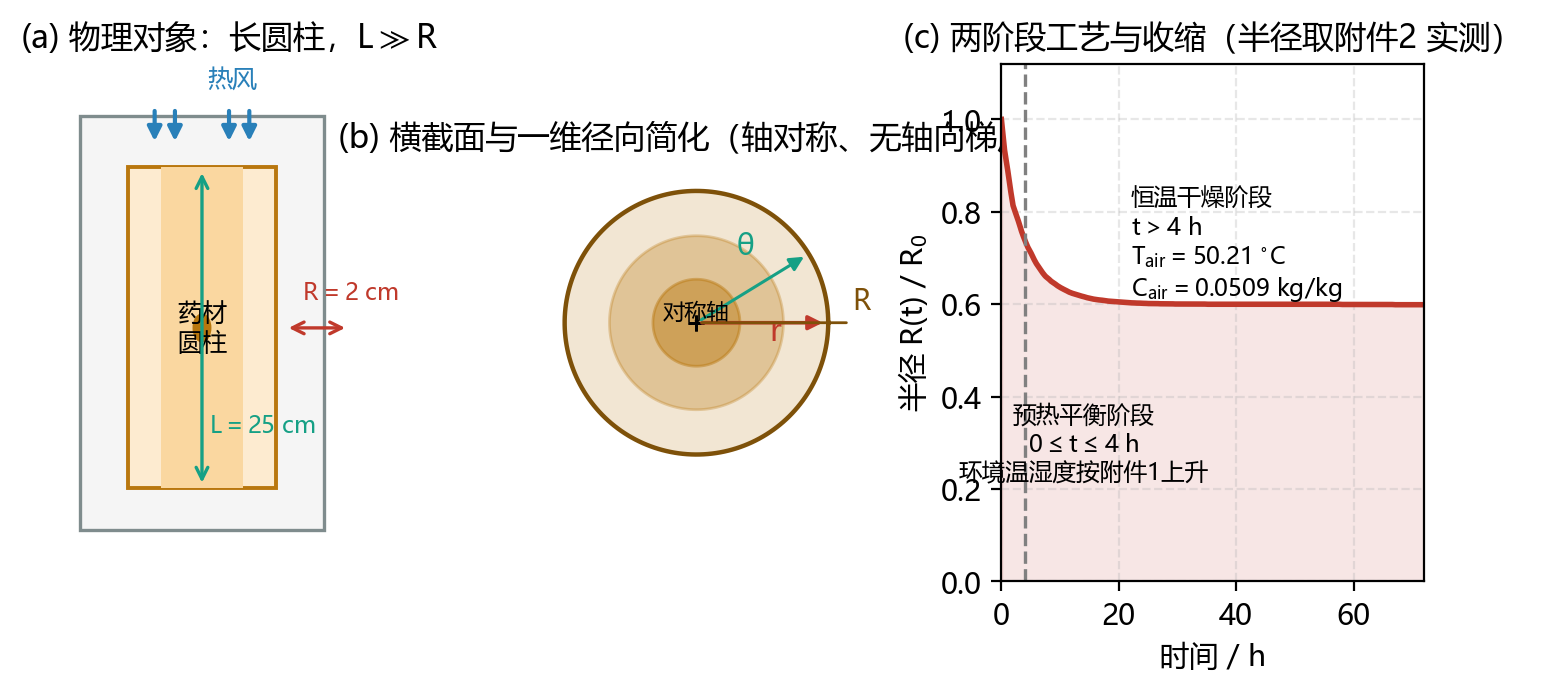
\includegraphics[width=0.84\textwidth]{figures/fig20_schematic.png}
  \caption{药材热风烘干问题的建模示意图：(a) 物理对象；(b) 横截面与一维径向简化；
  (c) 两阶段工艺与尺寸收缩}
  \label{fig:schematic}
\end{figure}

\subsection{传热控制方程}

在半径 $r$ 处取厚度 $\mathrm{d}r$、长 $L$ 的环形壳层。壳层内能的时变率等于
净导入的导热热流：

\[
\rho c_p\,(2\pi r L\,\mathrm{d}r)\frac{\partial T}{\partial t}
=-\Big[q_r\cdot 2\pi rL\Big]_{r}^{r+\mathrm{d}r},
\qquad q_r=-k\frac{\partial T}{\partial r},
\]

整理得圆柱坐标下的非稳态导热方程

\begin{equation}
\rho(C)\,c_p(C)\,\frac{\partial T}{\partial t}
=\frac{1}{r}\frac{\partial}{\partial r}\left(r\,k(C)\frac{\partial T}{\partial r}\right).
\label{eq:heat}
\end{equation}

\subsection{传质控制方程}

同一壳层内水分的时变率等于净导入的扩散质流。以干基浓度 $C$ 为变量，水分的
质量通量为 $j_r=-\rho_{d}D\,\partial C/\partial r$，其中 $\rho_d=\rho/(1+C)$ 为
单位湿体积内的干物质质量。注意到壳层内的干物质质量 $2\pi rL\rho_d\,\mathrm{d}r$
不随时间变化，对水分做守恒可得

\begin{equation}
\frac{\partial C}{\partial t}
=\frac{1}{r}\frac{\partial}{\partial r}\left(r\,D(C,T)\frac{\partial C}{\partial r}\right).
\label{eq:mass}
\end{equation}

式~\eqref{eq:mass} 的物理含义是：$C$ 是「每千克干物质的水量」，控制体随干物质
一起运动，因此方程中不含干物质密度的散度项，这也是后文处理收缩时的出发点。

\subsection{边界条件与初始条件}

\textbf{中心对称条件}（$r=0$）：

\begin{equation}
\left.\frac{\partial T}{\partial r}\right|_{r=0}=0,\qquad
\left.\frac{\partial C}{\partial r}\right|_{r=0}=0 .
\end{equation}

\textbf{表面 Robin 条件}（$r=R$，$n$ 取外法向）\cite{incropera2007}。热量由
热风以对流方式传入、水分由表面以对流方式带出：

\begin{equation}
-k\left.\frac{\partial T}{\partial r}\right|_{r=R}=h\left(T_s-T_{air}(t)\right),
\qquad
-D\left.\frac{\partial C}{\partial r}\right|_{r=R}=h_m\left(C_s-C_{air}(t)\right),
\label{eq:robin}
\end{equation}

其中 $T_s=T(R,t)$、$C_s=C(R,t)$。两式左端都是「向外法向的通量」，故 $T_{air}>T_s$
时导热项为负（热量向内传入），与 5.5 节的物质坐标形式的表面条件一致。

\textbf{初始条件}：

\begin{equation}
T(r,0)=28\,^\circ\mathrm{C},\qquad C(r,0)=2.55\ \mathrm{kg/kg},\qquad 0\le r\le R_0 .
\end{equation}

\subsection{收缩问题的物质坐标变换}

当 $R=R(t)$ 时，求解域随时间变化。引入物质坐标

\begin{equation}
\xi=\frac{r}{R(t)}\in[0,1],\qquad r=\xi R(t).
\end{equation}

对各向同性收缩，同一物质点在任意时刻满足 $r(t)=\xi R(t)$，即 $\xi$ 是材料标签。
干燥过程中干物质本身不迁移，故任一材料壳层 $[\xi,\xi+\mathrm{d}\xi]$ 所含的
干物质质量守恒。该壳层在当前构形下的体积（单位长度）为
$2\pi r\,\mathrm{d}r=2\pi R^2\xi\,\mathrm{d}\xi$，于是

\begin{equation}
\frac{\partial}{\partial t}\Big(\rho_d\,\xi R^2\Big)\Big|_{\xi}=0
\quad\Longrightarrow\quad
\rho_d(\xi,t)\,R(t)^2=\rho_d(\xi,0)\,R_0^2 ,
\label{eq:dryinv}
\end{equation}

即 $\rho_dR^2$ 是材料不变量——这是移动边界问题在物质坐标下的一个关键性质。

再对固定的材料区域 $[0,\xi]$ 做水分衡算。区域内水分只经由 $\xi$ 处的材料面与
外界交换：以干物质计的扩散质流密度为
$j_r=-\rho_dD\,\partial C/\partial r=-(\rho_dD/R)\,\partial C/\partial \xi$，
材料面面积（单位长度）为 $2\pi\xi R$。注意到区域内的干物质质量
$\mathrm{d}m_d=\rho_d\,2\pi R^2\xi'\,\mathrm{d}\xi'$ 不随时间改变，其中的水分
质量 $C\,\mathrm{d}m_d$ 的变化率即为 $\mathrm{d}m_d\,\partial_tC$，故

\begin{equation}
2\pi R^2\!\!\int_0^{\xi}\!\rho_d\,\xi'\,
\frac{\partial C}{\partial t}\,\mathrm{d}\xi'
=-\big(j_r\cdot2\pi\xi R\big)
=2\pi\,\xi\,\rho_d D\,\frac{\partial C}{\partial \xi}.
\end{equation}

两边对 $\xi$ 求导并约去公因子 $2\pi$，得物质坐标下的\textbf{一般形式}

\begin{equation}
\frac{\partial C}{\partial t}\bigg|_{\xi}
=\frac{1}{\xi R(t)^2\rho_d}\frac{\partial}{\partial \xi}
\left(\xi\,\rho_d D\frac{\partial C}{\partial \xi}\right).
\label{eq:shrink-general}
\end{equation}

由式~\eqref{eq:dryinv}，$\rho_d$ 沿 $\xi$ 的分布不随时间改变；而初始时刻
$C\equiv2.55$ kg/kg 处处相等，故 $\rho_d(\xi,0)$ 为常数。因此 $\rho_d$ 在
干燥全程都与 $\xi$ 无关，可从式~\eqref{eq:shrink-general} 中当作常数约去，
得到本文实际使用的形式

\begin{equation}
\boxed{\ \frac{\partial C}{\partial t}
=\frac{1}{\xi R(t)^2}\frac{\partial}{\partial \xi}
\left(\xi D\frac{\partial C}{\partial \xi}\right)\ }
\label{eq:shrink}
\end{equation}

\textbf{对流项严格为零}。这是本文处理收缩的核心结论：只要收缩是各向同性的，
在物质坐标下移动边界问题就化为固定域问题，只需把 $R(t)$ 代入 Laplacian 的
系数即可，无需引入网格运动或 ALE 对流项。当 $R(t)=R_0$ 时式~\eqref{eq:shrink}
退化为式~\eqref{eq:mass}，说明问题 1--4 可用同一套代码框架求解。

\textbf{推导前提}。上述推导用到两条前提，它们在本工况下成立，但应显式写出以免
误用。\textbf{（一）干基密度与 $\xi$ 无关}：这不是近似，而是式~\eqref{eq:dryinv}
的直接推论——$\rho_dR^2$ 逐材料点守恒，而初始含水率均匀使
$\rho_d(\xi,0)=\rho(C_0)/(1+C_0)$ 为常数，故 $\rho_d$ 全程与 $\xi$ 无关；它随
时间单调增大（附录 4 下 $C$ 由 $2.55$ 降到 $0$ 时 $\rho_d$ 由 $278.7$ 升到
$760$ kg/m$^3$），但该变化只依赖 $R(t)$，在式~\eqref{eq:shrink-general} 中被
约去。反之，若认为干密度随剖面不均匀，式~\eqref{eq:shrink} 会多出一阶项
$\frac{D}{R^2}\partial_\xi C\,\partial_\xi\ln\rho_d$，这种读法与附件 2 的实测
$R(t)$ 不相容（峰值偏差 $17.8\%$，10.6 节），故式~\eqref{eq:shrink} 在本工况下
是\textbf{精确}的。\textbf{（二）能量方程的单位体积热容}：本文直接取附录 4 的
$\rho(C)c_p(C)$ 作式~\eqref{eq:heat-shrink} 的系数，略去了「显热随含水率下降」
带来的附加项。其量级由 10.8 节的两个变体界定：把 $\rho c_p$ 乘 $(R_0/R)^2$ 后
$t_{dry}$ 只变 $+0.055\%$，加入体积项为 $-0.49\%$，都远小于 $D(C,T)$ 标定的
$\pm24\%$——因为水分场在 $2$ h 后已准平衡，这些项只改变温度的\emph{响应速率}，
不改变准平衡分布。用于收缩更剧烈（$R/R_0\ll0.6$）或热响应更慢的工况时，
上述前提应重新评估。

热传导方程在物质坐标下同理写成

\begin{equation}
\rho(C)c_p(C)\frac{\partial T}{\partial t}
=\frac{1}{\xi R(t)^2}\frac{\partial}{\partial \xi}
\left(\xi k(C)\frac{\partial T}{\partial \xi}\right).
\label{eq:heat-shrink}
\end{equation}

表面条件式~\eqref{eq:robin} 在物质坐标下为

\begin{equation}
-\frac{k}{R}\left.\frac{\partial T}{\partial \xi}\right|_{\xi=1}
=h\left(T_s-T_{air}\right),\qquad
-\frac{D}{R}\left.\frac{\partial C}{\partial \xi}\right|_{\xi=1}
=h_m\left(C_s-C_{air}\right).
\end{equation}

\subsection{物性经验关系与适用范围}

按题意，问题 1 用附录 2 的常数物性，问题 2--3 用附录 3 的经验式，问题 4 用
附录 4 的经验式（图~\ref{fig:props}）：

\begin{center}
{\small
\begin{tabular}{llll}
\toprule[1.2pt]
  & 附录 2（问题 1） & 附录 3（问题 2、3） & 附录 4（问题 4） \\
\midrule
$\rho$ / (kg/m$^3$) & $820$ & $650+128C$ & $760+90C$ \\
$c_p$ / (J/(kg$\cdot$K)) & $2600$ & $1450+2736\dfrac{C}{C+1}$ & $1850+2150\dfrac{C}{C+1}$ \\
$k$ / (W/(m$\cdot$K)) & $0.36$ & $0.21+0.38\dfrac{C}{C+1}$ & $0.12+0.20\dfrac{C}{C+1}$ \\
$D$ / (m$^2$/s) & $7\times10^{-9}e^{-0.89/C}$ & $2.4\times10^{-3}e^{-0.45/C}e^{-3850/T}$ & $4.2\times10^{-4}e^{-0.30/C}e^{-3850/T}$ \\
\bottomrule[1.2pt]
\end{tabular}
}
\end{center}

式中 $T$ 必须取绝对温度（K）。附录 2 的 $\rho,c_p,k$ 是常数、$D$ 又只依赖 $C$，
故\textbf{问题 1 的温度场与水分场完全解耦}（这也是 10.7 节环境口径只影响表面
水分浓度的原因）；问题 2--4 中 $D$ 依赖 $T$，两场才真正耦合。

\begin{figure}[htbp]
  \centering
  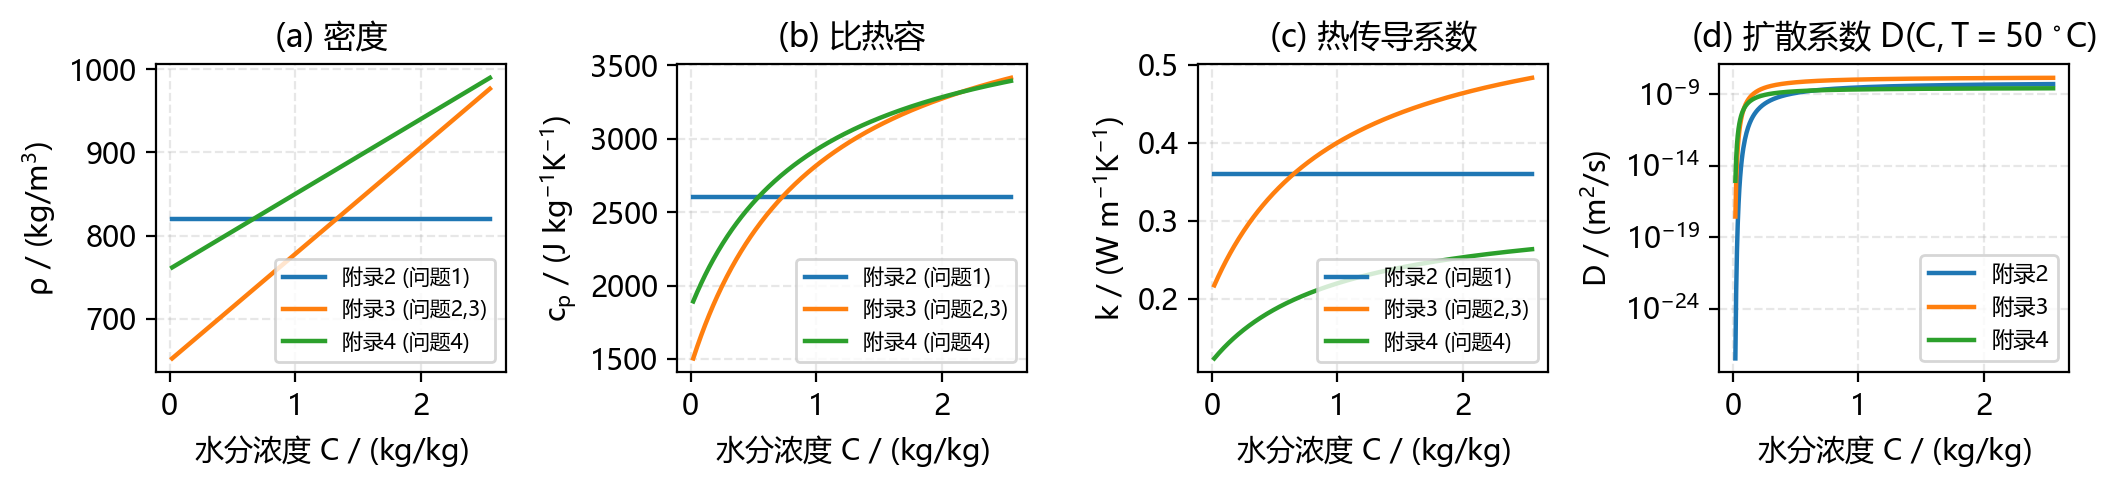
\includegraphics[width=0.84\textwidth]{figures/fig06_properties.png}
  \caption{附录给出的物性经验关系随水分浓度的变化}
  \label{fig:props}
\end{figure}

\textbf{量纲与数量级检查}。$e^{-3850/T}$ 是 Arrhenius 因子，对应活化能
$E_a=3850R_g=3850\times8.314=32.0$ kJ/mol（$R_g$ 为气体常数）；干燥中有效
水分扩散系数随温度呈 Arrhenius 形式是常用假设\cite{karatas1997}。
$e^{-a/C}$ 项则体现「随含水率下降扩散阻力急剧增大」的降速干燥特征。
由附录 3 计算：$C=2.55$、$T=50\,^\circ$C 时 $D=1.35\times10^{-8}$ m$^2$/s；
$C=0.15$ 时 $D=8.0\times10^{-10}$ m$^2$/s，下降 17 倍，说明\textbf{干燥后期
由内部扩散控制}。\textit{适用范围说明}：上述经验式由题目给定，其标定区间未在
题面说明；当 $C\to0$ 时 $e^{-a/C}\to0$，公式在极低含水率下会给出过小的 $D$，
本文据此在程序中设 $C\ge10^{-3}$ kg/kg 的下限保护，并在灵敏度分析中量化
$a$ 与 $3850$ 的不确定性影响。

\subsection{无量纲分析与工作量级的先验判断}

定义热 Biot 数、传质 Biot 数、Fourier 数与 Lewis 数：

\begin{equation}
Bi=\frac{hR_0}{k},\quad Bi_m=\frac{h_mR_0}{D},\quad
Fo=\frac{\alpha t}{R_0^2},\quad \mathrm{Le}=\frac{D}{\alpha}.
\end{equation}

\begin{itemize}
  \item 问题 1：$Bi=1.389$，$Bi_m=3.24$，$\mathrm{Le}=2.9\times10^{-2}$，
  $Fo_T(1800\,\mathrm{s})=0.760$，$Fo_D(1800\,\mathrm{s})=0.0222$。
  \item 问题 3（取 $C=2.55$、$T=50\,^\circ$C）：$D=1.347\times10^{-8}$ m$^2$/s，
  $\alpha=k/(\rho c_p)=0.4830/(976.4\times3415.3)=1.448\times10^{-7}$ m$^2$/s，
  $\mathrm{Le}=D/\alpha=0.093$，$Bi_m=h_mR_0/D=1.19$。
\end{itemize}

\textbf{两条先验结论}（图~\ref{fig:regime}）：第一，$Fo_D\ll Fo_T$，即温度先于
水分达到准平衡，因此问题 1 的 30 分钟内「水分几乎不动、温度显著上升」；
第二，$Bi_m$ 量级为 1，说明内部扩散与外部对流传质阻力\textbf{相当}，
不能简单地把表面当作平衡边界处理，必须保留 Robin 条件。

\begin{figure}[htbp]
  \centering
  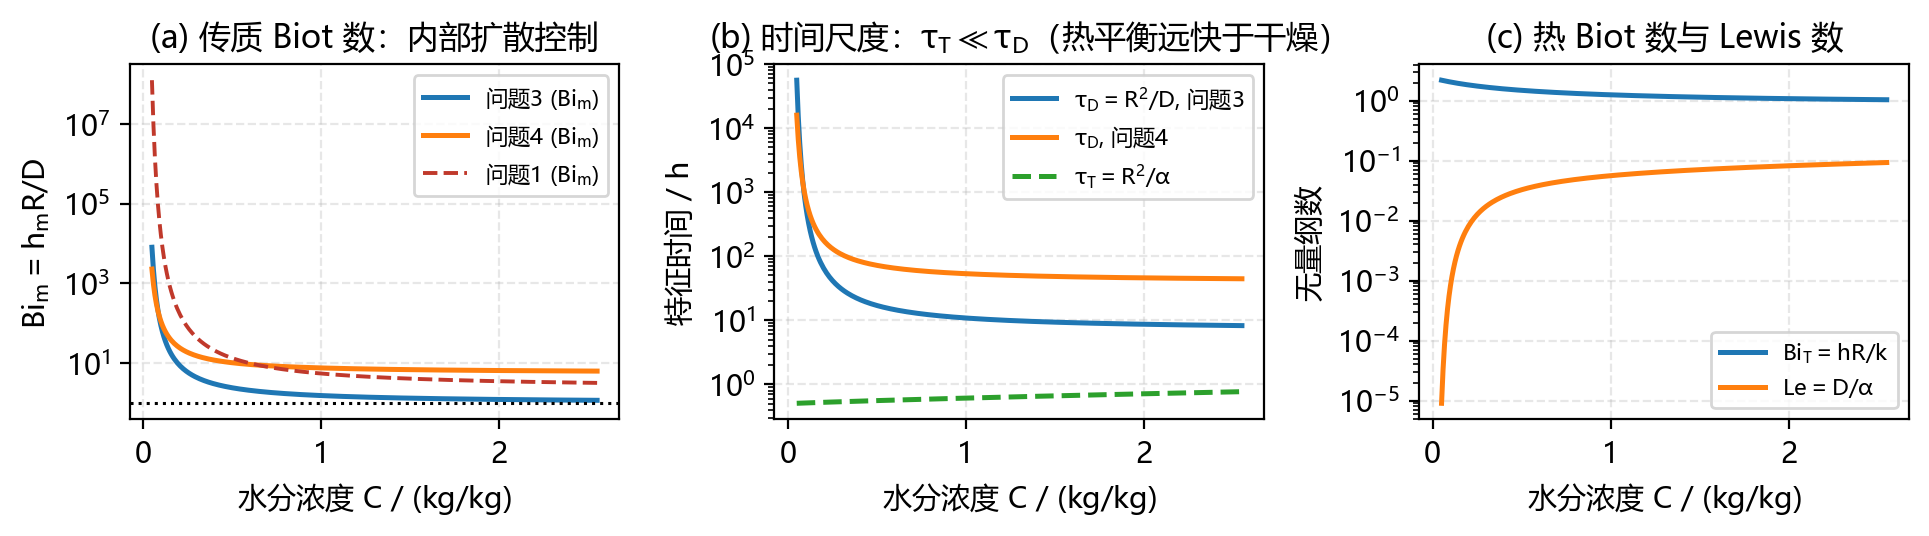
\includegraphics[width=0.84\textwidth]{figures/fig21_regime.png}
  \caption{无量纲分析：模型所处的工作区间。(a) 传质 Biot 数；(b) 各特征时间尺度；
  (c) 热 Biot 数与 Lewis 数}
  \label{fig:regime}
\end{figure}

\subsection{数值方法}

\textbf{空间离散}。在 $\xi\in[0,1]$ 上取 $N+1$ 个节点
$\xi_i=ih$，$h=1/N$，采用\textbf{节点中心有限体积}格式：节点 0 位于对称轴、
节点 $N$ 恰好位于药材表面。控制体取 $[0,h/2]$、$[\xi_i-h/2,\xi_i+h/2]$ 与
$[1-h/2,1]$，对应的体积测度为

\[
\mathrm{vol}_0=\frac{h^2}{8},\qquad
\mathrm{vol}_i=\xi_i h\ (1\le i\le N-1),\qquad
\mathrm{vol}_N=\frac{h}{2}-\frac{h^2}{8}.
\]

将式~\eqref{eq:shrink} 在控制体上积分，记面通量 $g=\xi D\partial_\xi C$，得

\begin{equation}
\frac{\mathrm{d}C_i}{\mathrm{d}t}
=\frac{1}{R^2\,\mathrm{vol}_i}\left(g_{i+\frac12}-g_{i-\frac12}\right),\qquad
g_{i+\frac12}=\frac{\xi_{i+\frac12}D_{i+\frac12}}{h}\left(C_{i+1}-C_i\right),
\end{equation}

其中面扩散系数取相邻两节点的\textbf{算术平均}
$D_{i+1/2}=(D_i+D_{i+1})/2$。表面面通量
由式~\eqref{eq:robin} 给出：$g_{N+\frac12}=-R\,h_m(C_N-C_{air})$；轴心处
$g_{-\frac12}=0$。该格式\textbf{逐项守恒}：对所有控制体求和可得水分总量的
变化率恰等于表面通量，误差仅为舍入误差。

\textbf{时间离散}。物性系数取上一时间步的显式值，未知量隐式处理，采用
$\theta$ 法：

\begin{equation}
\left(I-\Delta t\,\theta\,L\right)\phi^{n+1}
=\left(I+\Delta t(1-\theta)L\right)\phi^{n}+\Delta t\,\theta\,\mathbf{c},
\end{equation}

其中 $L$ 为空间离散算子，$\mathbf{c}$ 为环境边界带来的常数项。取
$\theta=1/2$ 即 Crank--Nicolson，时间精度二阶；但初始时刻表面条件存在跳跃
（$C_s=2.55$ 而 $C_{air}=0.0196$），Crank--Nicolson 对最高频空间模态几乎不
衰减（$|g|\to1$），会产生非物理振荡，故\textbf{前 4 步改用 $\theta=1$
（Rannacher 启动）}。每步只需求解两个三对角线性系统（Thomas 算法），
$N=1600$ 时单步约 0.5 ms。

\textbf{输出与插值}。节点中心格式在 $\xi=1$ 处恰好存放表面值，无需外推；
其余输出位置用三点 Lagrange 二次插值，$\xi=0$ 处利用偶对称性
$C(\xi)=C(0)+a\xi^2$ 由前两个节点推定。

\textbf{网格与步长}。经收敛性研究（见检验章节）确定生产设置为
$N=1600$。时间步长的取法两个问题群不同：\textbf{问题 1} 全程 $1800$ s 都取
$\Delta t=1$ s；\textbf{问题 2--4} 时间跨度达 $72$ h，在热瞬变最强的前 $7200$ s
取 $\Delta t=1$ s，之后放宽到 $\Delta t=10$ s，输出仍插值到整数秒。
两档步长在 $N=800$ 上给出的 $t_{dry}$ 相差 $13.6$ s（$0.0066\%$，10.2 节），
故该切换不引入可分辨误差。
